\documentclass[tikz,border=5pt]{standalone}
\usetikzlibrary{shapes, shapes.geometric}

\begin{document}

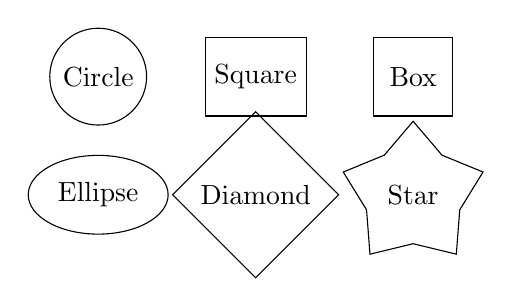
\begin{tikzpicture}
% 圆形节点
\node[circle, draw, minimum size=1cm] (A) at (0,0) {Circle};

% 方形节点
\node[rectangle, draw, minimum size=1cm] (B) at (2,0) {Square};

% 正方形（更精确）
\node[rectangle, draw, minimum width=1cm, minimum height=1cm] (C) at (4,0) {Box};

% 其他形状
\node[ellipse, draw, minimum size=1cm] (D) at (0,-1.5) {Ellipse};
\node[diamond, draw, minimum size=1cm] (E) at (2,-1.5) {Diamond};
\node[star, draw, minimum size=1cm] (F) at (4,-1.5) {Star};

\end{tikzpicture}

\end{document}